%%
%% This is file `lexample.tex',
%% Sample file for siam macros for use with LaTeX 2e
%%
%% October 1, 1995
%%
%% Version 1.0
%%
%% You are not allowed to change this file.
%%
%% You are allowed to distribute this file under the condition that
%% it is distributed together with all of the files in the siam macro
%% distribution. These are:
%%
%%  siamltex.cls (main LaTeX macro file for SIAM)
%%  siamltex.sty (includes siamltex.cls for compatibility mode)
%%  siam10.clo   (size option for 10pt papers)
%%  subeqn.clo   (allows equation numbners with lettered subelements)
%%  siam.bst     (bibliographic style file for BibTeX)
%%  docultex.tex (documentation file)
%%  lexample.tex (this file)
%%
%% If you receive only some of these files from someone, complain!
%%
%% You are NOT ALLOWED to distribute this file alone. You are NOT
%% ALLOWED to take money for the distribution or use of either this
%% file or a changed version, except for a nominal charge for copying
%% etc.
%% \CharacterTable
%%  {Upper-case    \A\B\C\D\E\F\G\H\I\J\K\L\M\N\O\P\Q\R\S\T\U\V\W\X\Y\Z
%%   Lower-case    \a\b\c\d\e\f\g\h\i\j\k\l\m\n\o\p\q\r\s\t\u\v\w\x\y\z
%%   Digits        \0\1\2\3\4\5\6\7\8\9
%%   Exclamation   \!     Double quote  \"     Hash (number) \#
%%   Dollar        \$     Percent       \%     Ampersand     \&
%%   Acute accent  \'     Left paren    \(     Right paren   \)
%%   Asterisk      \*     Plus          \+     Comma         \,
%%   Minus         \-     Point         \.     Solidus       \/
%%   Colon         \:     Semicolon     \;     Less than     \<
%%   Equals        \=     Greater than  \>     Question mark \?
%%   Commercial at \@     Left bracket  \[     Backslash     \\
%%   Right bracket \]     Circumflex    \^     Underscore    \_
%%   Grave accent  \`     Left brace    \{     Vertical bar  \|
%%   Right brace   \}     Tilde         \~}


\documentclass[final]{siamltex}

% definitions used by included articles, reproduced here for
% educational benefit, and to minimize alterations needed to be made
% in developing this sample file.

\newcommand{\pe}{\psi}
\def\d{\delta}
\def\ds{\displaystyle}
\def\e{{\epsilon}}
\def\eb{\bar{\eta}}
\def\enorm#1{\|#1\|_2}
\def\Fp{F^\prime}
\def\fishpack{{FISHPACK}}
\def\fortran{{FORTRAN}}
\def\gmres{{GMRES}}
\def\gmresm{{\rm GMRES($m$)}}
\def\Kc{{\cal K}}
\def\norm#1{\|#1\|}
\def\wb{{\bar w}}
\def\zb{{\bar z}}

% some definitions of bold math italics to make typing easier.
% They are used in the corollary.

\def\bfE{\mbox{\boldmath$E$}}
\def\bfG{\mbox{\boldmath$G$}}


%%%%%%%%%%%%%%%%%%%%%%%%%%%%%%%%%%%%%%
% Actual stuff starts here


%% encoding
\usepackage[utf8]{inputenc}
\usepackage[english]{babel}


%% Math packages
\usepackage{amsmath}
\usepackage{amsfonts}
\usepackage{amssymb}
\usepackage{mathrsfs}

\usepackage{color}
\usepackage{hyperref}
\usepackage{graphicx}
\usepackage{listings}

\newcommand{\mycomment}[1]{{\color{blue} #1}}

\title{Probabilistic Program Induction for Model-Based Reinforcement Learning}

% The thanks line in the title should be filled in if there is
% any support acknowledgement for the overall work to be included
% This \thanks is also used for the received by date info, but
% authors are not expected to provide this.

\author{Zenna Tavares and Max Siegel\thanks{Department of Brain \& Cognitive Sciences, Massachusetts Institute of Technology}
}
\begin{document}

\maketitle

\begin{abstract}
Model-based reinforcement learning (RL) is a powerful method for acting in unknown environments, but most approaches require specific, limiting assumptions about the world model.
Probabilistic program induction promises flexible, universal learning from data.
We present an outline of a method for inducing and using adaptive generative models in reinforcement learning. 
The approach is to learn probabilistic programs from experience and choose actions by sparse sampling.
We describe several systems that we have built towards this goal. 
RL-Church is a system based on the Church programming language that allows for easy specification of complex generative models in RL tasks.
Stochastic Javascript is a extension of Javascript which allows for fast computation and easy Internet data collection. These tools aid development of improved RL agents.
\end{abstract}

\begin{keywords}
Probabilistic program induction, model-based reinforcement learning, Church, Stochastic Javascript
\end{keywords}

\section{Introduction}
Reinforcement learning (RL) is a successful field of machine learning that has enjoyed much practical application, and is often the method of choice when acting in unknown or partially-unknown environments.

However, there are simple examples of problems that humans solve effortlessly but pose challenges for standard RL algorithms. Consider the finite-state automaton in Figure 1.
We made this agent with church and he learned everything.
Well done, agent.

However, there are simple examples of problems that humans solve effortlessly but pose challenges for standard RL algorithms. 
Consider the finite-state automaton in Figure 1 (drawn from \cite{Dearden98-bayesianq-learning}).\begin{figure}
\begin{center}

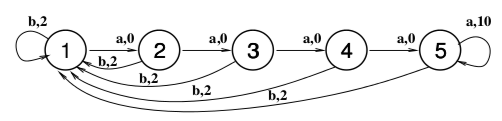
\includegraphics[scale=.4]{chain}

\end{center}
\caption{The chain problem; with probability .2, each action \emph{a} or \emph{b} results in a transition to the starting state 1. State 5 gives much greater reward than state 1, but standard RL algorithms fail to discover it.}
\end{figure}
The task is difficult because before the agent reaches the fifth stage, all of the evidence received suggests that the best strategy is to remain at the first state.
Yet it seems clear that the potential rewards are sufficient to warrant visiting each state.
This is an example of the \emph{exploration-exploitation tradeoff}: to maximize final reward, when should one decide to quit roaming and settle down?

Recent work has shown that humans perform very well on the chain problem, finding the best state hundreds or thousands of times faster than most RL algorithms.

What could account for such dramatic differences?
Humans seem to perform very well on problems with clear structure, possessing a strong inductive bias towards simplicity.
Conversely, human performance is very poor in general RL environments. 

To capture this apparent feature of human learning, we used techniques from Bayesian RL and probabilistic program induction to create a principled, (semi-) tractable method for learning to act in unknown environments. 
Church is a probabilistic programming language that allows for flexible, compositional representation of generative models. 
Since its release, there has been steadily increasing interest in Bayesian program induction using Church.
Most of this work uses a program length prior to learn concise models from data.
This framework seems well suited to the problem at hand; the length prior prefers structured models that abstract over states and actions, without specifying their precise form.

Both probabilistic programming and Bayesian RL pose significant computational difficulties. Bayesian RL requires that one maintain a posterior distribution over possible world models, which we represent using Church programs. 
Exact action selection in Bayesian RL requires exact planning, which is impossible for infinite horizon problems and intractable for finite horizon problems.
We use sparse sampling for action selection, which maintains our Bayesian approach while making planning tractable.
Finally, probabilistic program induction is perhaps the most difficult computational task that we face; calculating the posterior probability of programs is intractable. 
We use two strategies to enable computation.
Rather than attempt to model the posterior probability directly, we draw (approximate) samples from the posterior distribution; this is a ubiquitous strategy in machine learning and computational statistics. 
To find high-probability programs, we use heuristics that favor abstraction (drawn from :::::Hwang et al::::).

The plan of the paper is as follows. 
In Section 2, we review background material. 
In Section 3, we outline our proposed method. 
In Section 4, we describe RL-Church, a RL system based on the Church programming language. 
In Section 5, we describe Stochastic Javascript, an extension of the Javascript programming language.
To conclude, we discuss possible applications and future research directions.
\section{Background}

\section{Stochastic Javascript}
To meet the resource requirements of both reinforcement learning and program induction we developed a stochastic extension of the JavaScript programming language.
JavaScript is a dynamic and weakly typed multi-paradigm language, with C-like syntax.
In spite of its name, it bears little semantic resemblance to Java and instead derives many of its ideas from Scheme, with support for first class functions, closures, lambda expressions and an $eval$ procedure to evaluate dynamically generated code.
It also offers many of the features associated with more commonly used imperative languages, such as a prototypical object model, the modification of state, and the ability to introduce side-effects in functions.

Competition between browser vendors has in recent years taken place on the performance front, leading to a tremendous increase in the speed of JavaScript implementations, which now routinely outperform other interpreted languages in benchmark tests.
A large contribution to this progress stems from the adoption of just-in-time compilation (JIT) techniques, which sits somewhere in between interpretation and static (ahead-of-time) compilation.
In JIT compilers

This combination of language and implementation properties make JavaScript particularly attractive for this kind of domain

Due to JIT and other run-time optimisations, anecdotal evidence has even demonstrated JavaScript outperforming natively compiled code for certain classes of task.
Program induction



\lstset{language=C++}
\begin{verbatim}
var genExp = function() {
	if (flip(0.4)) {
		return [flip(0.5) ? ["add",2]:["minus",2]].concat(genExp(),genExp());
	}
	else {
		return [[1 + sampleInteger(10),-1]];
	}
}
\end{verbatim}
>>>>>>> 63a090b9623fbd3789e240fb9ecbeedcf5dea43d

\bibliographystyle{siam}
\bibliography{induct}

\end{document}
